\documentclass[12pt,oneside]{fithesis2}
\usepackage{graphicx}
\usepackage[english]{babel}       % Multilingual support
\usepackage[utf8]{inputenc}       % UTF-8 encoding
\usepackage[T1]{fontenc}          % T1 font encoding
\usepackage[                      % A sans serif font that blends well with Palatino
  scaled=0.86
]{berasans}
\usepackage[                      % A tt font if you do not like LM's tt
  scaled=1.03
]{inconsolata}
\usepackage{blindtext}
\usepackage[hyphens]{url}
\usepackage[                      % Clickable links
  plainpages = false,               % We have multiple page numberings
  pdfpagelabels                     % Generate pdf page labels
]{hyperref}            % Lorem ipsum generator
\usepackage{listings}
\lstset{frame=lrtb, captionpos=b, breaklines=true, literate={\\\-}{}{0\discretionary{-}{}{}}}
\usepackage{multicol}
\usepackage{enumitem}

\thesislang{en}                   % The language of the thesis
\thesistitle{Extend WildFly Application Server logging capabilities}       % The title of the thesis
\thesissubtitle{Diploma Thesis}  % The type of the thesis
\thesisstudent{Bc. Radek Koubský}          % Your name
\thesiswoman{true}                % Your gender
\thesisfaculty{fi}                % Your faculty
\thesisyear{\the\year}     % The academic term of your thesis defense
\thesisadvisor{RNDr. Adam Rambousek, Ph.D.}   % Your advisor

\begin{document}
  \FrontMatter                    % The front matter
    \ThesisTitlePage                % The title page
    \begin{ThesisDeclaration}       % The declaration
      \DeclarationText
      \AdvisorName
    \end{ThesisDeclaration}
    \begin{ThesisThanks}            % The acknowledgements (optional)
      I would like to thank my supervisor\,\dots
    \end{ThesisThanks}
    \begin{ThesisAbstract}          % The abstract
      The aim of the bachelor work is to provide\,\dots
    \end{ThesisAbstract}
    \begin{ThesisKeyWords}          % The keywords
      keyword1, keyword2\,\dots
    \end{ThesisKeyWords}
    \tableofcontents                % The table of contents
%   \listoftables                   % The list of tables (optional)
%   \listoffigures                  % The list of figures (optional)
  
  \MainMatter                     % The main matter
    \chapter{Introduction}   
    
\chapter{Wildfly}
\label{wildfly_chapter}
In this chapter, the \textit{Wildfly Application Server} (former JBoss AS) is described. Because of the server complexity, only specific part are mentioned and description of its internal structure and configuration is provided. Further information about Wildfly can be found at official website \url{http://wildfly.org/}. Wildfly 8 Documetation \cite{wildfly_doc} is used as the main source for this chapter.

Wildfly is one of the leading application servers in the area of enterprise solutions. From \cite[Getting Started with WildFly 8]{wildfly_doc}: ''WildFly 8 is an exceptionally fast, lightweight and powerful implementation of the Java Enterprise Edition 7 Platform specifications.'' The Wildfly project is licensed as \textit{Open Source} and supported by the \textit{JBoss Community}. However, there is commercial version of Wildfly, \textit{JBoss Enterprise Application Platform}, which is licensed and supported by Red Hat.

\section{Structure of Wildfly}
The structure of Wildfly has been changed in recent years due to requirements on maintainability and performance. Wildfly is formed by the wildfly core and set of subsystems. Subsystems are defined as on-demand services which are called by applications deployed on the server. Each subsystem is responsible for specific functionality.

The core of the server was significantly changed in the version JBoss AS 7. It consists of two parts \cite{jboss_as_book}:

\begin{itemize}
	\item \textbf{JBoss Modules}: ''This handles the class loading of resources in the container.
	You can think of JBoss Modules as a thin bootstrap wrapper for executing
	an application in a modular environment.''
	\item \textbf{Modular Service Container (MSC)}: ''This provides a way to install,
	uninstall, and manage the services used by a container. MSC further
	enables the injection of resources into services and dependency
	management between services.''
\end{itemize}

The structure of the core described above has remained to the last version of Wildfly. The following diagram illustrates basic architecture of the Wildfly core:

\begin{figure}[ht!]
	\centering
	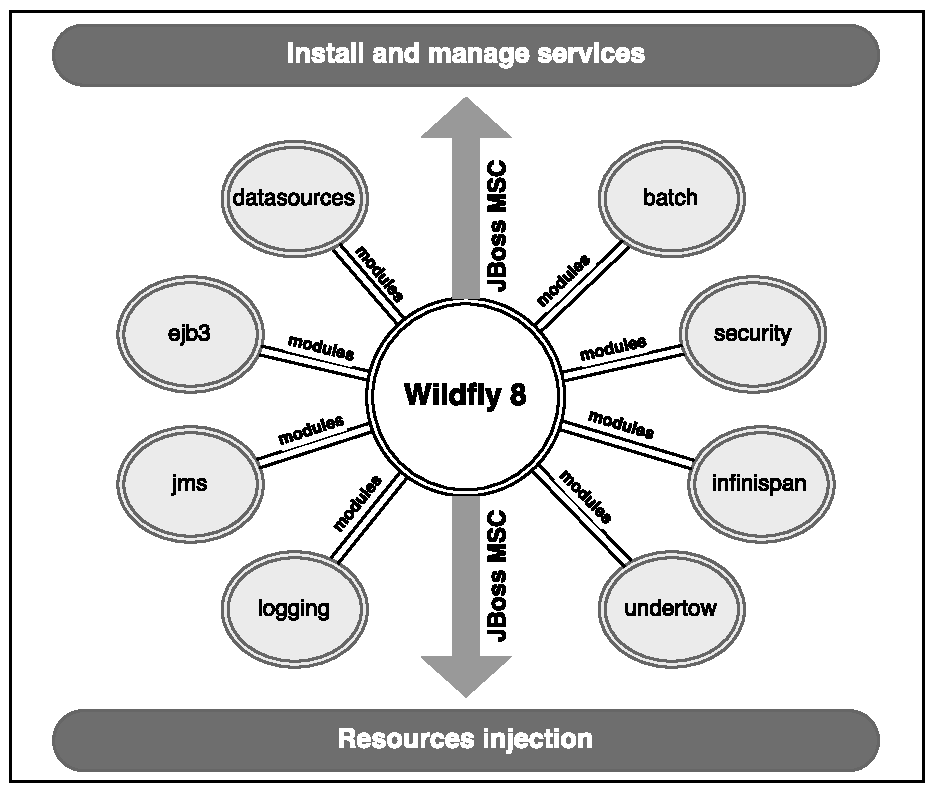
\includegraphics[width=\textwidth]{images/wildfly_core}
	\caption{Wildfly core architecture \cite{wildfly_book}}
	\label{wildfly_core}
\end{figure}

\section{JBoss Modules}
\label{jboss_modules_sec}
Class loading is problematic domain in the context of application servers. Wildfly comes with the \textit{JBoss Modules} class loading system which provides effective way of loading classes into class path. \textit{JBoss Modules} is defined as follows \cite[Introduction]{jboss_modules_doc}: ''JBoss Modules is a standalone implementation of a modular (non-hierarchical) class loading and execution environment for Java.''

\textit{JBoss Modules} is implemented as delegating class loader model which is thread-safe, fast, and highly concurrent. Each \textit{JAR} which is loaded into class path is handled as a \textit{module}. A module must define list of dependencies only to modules it depends on. Modules are loaded only on request by an application, thus the performance of the application is dependent on modules which are currently used by the application.

Wildfly defines two types of modules \cite{wildfly_book}:

\begin{itemize}
	\item Static modules
	\item Dynamic modules
\end{itemize}

The following diagram shows architecture of static and dynamic modules:

\begin{figure}[ht!]
	\centering
	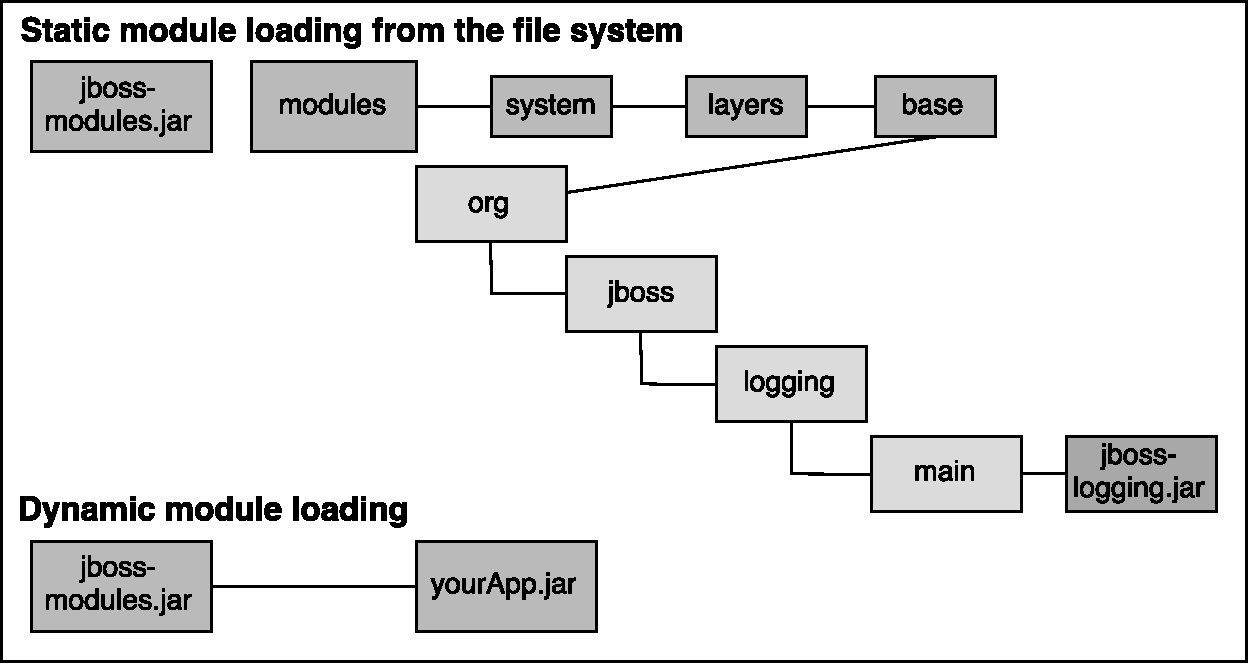
\includegraphics[width=\textwidth]{images/jboss_modules}
	\caption{JBoss modules architecture \cite{wildfly_book}}
	\label{jboss_modules_image}
\end{figure}

Static modules are defined in form of hierarchical directory structure. In Wildfly 8, static modules are located within \textit{JBOSS\_HOME/modules/system/layers/base} directory. A directory structure of a module is derived from the name and version of the module. The specific directory of the module contains module descriptor and resources required by the module (\textit{JAR} files).

The module descriptor is represented by \textit{module.xml} file. The following example shows module descriptor of the \textit{javax.batch.api module.xml} module:
\begin{lstlisting}[caption = Example of a module descriptor \cite{wildfly_book}, label = module_descriptor, language=XML]
<module xmlns="urn:jboss:module:1.3" name="javax.batch.api">
 <resources>
  <resource-root path="jboss-batch-api_1.0_spec-1.0.0.Final.jar"/>
 </resources>
 <dependencies>
  <module name="javax.api"/>
  <module name="javax.enterprise.api"/>
 </dependencies>    
</module>
\end{lstlisting}
\noindent	
The root \verb|<module>| element defines resources and dependencies of the module. 

Resources are defined within the \verb|<resources>| element which contains one or more \verb|resource-root>| elements. Each \verb|<resource-root>| element has the \textit{path} attribute which specifies path to the \textit{JAR} file. The example above uses only one resource, the \textit{jboss-batch-api\_1.0\_spec-1.0.0.Final.jar} file located in the module directory next to the \textit{module.xml} file.

The next element, \verb|<dependencies>|, is used to define dependencies for a module. A dependency is defined by the \verb|<module>| element which identifies specific module in the hierarchical directory structure. In the example above, \textit{javax.api} and \textit{javax.enterprise.api} modules will be resolved in the name resolution process as dependencies for the \textit{javax.batch.api} module.

Dynamic modules are defined for each deployment of an application. There are two approaches how to create dynamic module \cite{wildfly_book}.

First option is to define dependencies within a file called \textit{MANIFEST} which is placed in a \textit{JAR} file of an application. Dependencies of a \textit{JAR} file are defined in the \textit{Dependencies} header; each dependency is separated by comma. The following line is an example of a \textit{MANIFEST} file with one dependency:

\begin{lstlisting}[frame=]
Dependencies: org.jboss.logging
\end{lstlisting}

\newpage
The second option is to configure \textit{deployment-structure.xml} by adding module dependency to it:

\begin{lstlisting}[caption = Configuring deployment structure file \cite{wildfly_book}, label = dynamic_module_descriptor, language=XML]
<jboss-deployment-structure>
 <deployment>
  <dependencies>
   <module name="org.jboss.logging" />
  </dependencies>
 </deployment>
</jboss-deployment-structure>
\end{lstlisting}

\section{Wildfly logging subsystem}
\label{wildfly_logging}
Logging subsystem is responsible for displaying all logs which appear in the application server i.e. in every subsystem and user applications. The logging subsystem consists of the following parts: \textit{handler configurations}, \textit{logger}, \textit{the root logger declarations} and \textit{logging profiles}. Loggers declare set of handlers which send logs to defined destinations such as console, a file, network and others \cite[Logging Configuration]{wildfly_doc}.

The logging configuration can be defined in XML files (standalone.xml, domain.xml etc.), web console or command line interface. The following example illustrates a snippet of logging subsystem configuration from XML configuration file:

\begin{lstlisting}[caption = Configuring logging subsystem, label = logging_subsystem, language=XML]
<subsystem xmlns="urn:jboss:domain:logging:1.0">
 <console-handler name="CONSOLE" autoflush="true">
  <level name="DEBUG"/>
  <formatter>
   <pattern-formatter pattern="%d{HH:mm:ss,SSS} %-5p [%c] (%t) %s%E%n"/>
  </formatter>
 </console-handler>
 <logger category="com.arjuna">
  <level name="WARN"/>
 </logger>
 <root-logger>
  <level name="DEBUG"/>
   <handlers>
    <handler name="CONSOLE"/>
   </handlers>
 </root-logger>
</subsystem>
\end{lstlisting}
\noindent
The \verb|<console-handler>| element identifies a handler which prints logs from Wildfly to a console. Handler element contains two child elements, the \verb|<level>| and the \verb|<formatter>| element. The level element specifies a log level the outgoing logs must match. The formatter element defines output format for logs in the console.

The \verb|<logger>| element defines a logger and its level for specific package or class. Target package or class is specified by the \textit{category} attribute.

The \verb|<root-logger>| element is same as the logger element only it does not have the category attribute as it is the root logger.


\subsection{Loggers}
Log messages are created by loggers. Definition of a logger consists of a category which is represented by package or class name. Whenever the logger tries to log a message, it first checks the level of the message. If the level of the message is greater than the level of the logger, a filter is applied to the log message.  A filter determines whether the log message is loggable or not according to filter rule. The logging subsystem provides rich set of rules (expressions) for filters; detailed description of all rules can be found in the Logging documentation \cite[Logging Configuration]{wildfly_doc}.

Wildfly logging subsystem defines the following set of logger levels \cite[Logging Configuration]{wildfly_doc}:

\begin{multicols}{2}
	\begin{itemize}
		\item TRACE
		\item DEBUG
		\item FINE
		\item INFO
		\item WARN
		\item ERROR
		\item SEVERE
		\item OFF
	\end{itemize}
\end{multicols}

\subsection{Handlers}
\label{handlers}
Handlers represent next step in the log processing. If a log message is loggable, a handler processes the message e.g. sends the message to system console or stores the message to a file.

Logging subsystem provides the following set of handlers \cite[Logging Configuration]{wildfly_doc}:
\begin{itemize}
	\item async-handler
	\item console-handler
	\item file-handler
	\item periodic-rotating-file-handler
	\item size-rotating-file-handler
	\item syslog-handler
\end{itemize}
\noindent
However, a custom handler can be implemented for user specific requirements.

\subsection{Defining custom handler}
\label{custom_handler}
Logging subsystem provides straightforward process of custom handler implementation. A custom handler is standard module in the JBoss Modules architecture \ref{jboss_modules_sec}.

The simplest way to create a custom handler is to extend \textit{java.util.logging.Handler} class which is part of \textit{Java Logging API}. The \textit{Java Logging API} provides standard log handler lifecycle which is used to built a custom handler.

The following example shows custom handler class \textit{MyHandler.java}:
\begin{lstlisting}[caption = Custom handler class, label = custom_handler_class, language=Java]
package com.examples.logging
public class MyHandler extends Handler {
	@Override
	public void publish(LogRecord record) {
		//do something with log
	}
	
	@Override
	public void flush() ...
	@Override
	public void close() ...
}
\end{lstlisting}
\noindent
The next step in custom handler implementation is to create \textit{module.xml} file with proper configuration according to \ref{module_descriptor}. Then the \textit{myHandler.jar} with the \textit{module.xml} file is placed to specific module directory, for example \textit{JBOSS\_HOME/modules/system/layers/base/com/examples/myhandler/main}.
\noindent
Final step of the custom handler implementation is to add the custom handler to the logging subsystem configuration:
\begin{lstlisting}[caption = Adding custom handler to the logging subsystem configuration, label = custom_handler_logging_subsystem, language=XML]
 <custom-handler name="MyHandler" class="com.examples.logging.MyHandler" module="com.examples.myhandler">
  <level name="DEBUG"/>
 <formatter>...</formatter>
 </custom-handler>
\end{lstlisting}
\noindent
After all previous steps, the \textit{MyHandler} will be used to process log messages in Wildfly.

\chapter{Byteman}
\label{byteman_chap}
This chapter aims to introduce \textit{Byteman}, a bytecode manipulation tool, and its use in Java applications. Fundamental principles, functions, and structure of Byteman are described.
At the end of the chapter, an example of simple java application is provided in order to understand bytecode injection which Byteman uses. More detailed documentation, tutorials, and guidelines 
which cover almost every aspect of Byteman can be found in different versions at official website \url{http://byteman.jboss.org/}. Primary source for this thesis is Byteman documentation 3.0.0 \cite{byteman_doc}.

\section{Introduction to Byteman}
Byteman is a bytecode manipulation tool which uses bytecode injection\footnote{Bytecode injection (or bytecode instrumentation) is a process of modifying the actual bytecode of a class.} in order to change a java application as it is being loaded by \textit{Java virtual machine} or while the application is running \cite[Introduction to Byteman]{byteman_doc}.

Because of the bytecode injection, there is no need to change the original source code nor to recompile or redeploy the application itself. In other words, it is possible to add, replace or remove injected code at runtime without interrupting a Java application. Byteman also provides a way to inject code into the Java language by modifying classes such as \textit{java.lang.Thread} and other classes from \textit{java.lang} package. Byteman uses simple scripting language called \textit{Event Condition Action} (\ref{subsec:eca_sec}) rules to determine how the original Java code should be transformed according to event and condition.

The original purpose of Byteman was to provide a mechanism for automation tests used in multi-threaded and multi-JVM Java applications using a technique called fault injection. Byteman can be used to inject faults which cause an application to invoke unusual or unexpected methods which are required for certain test scenarios. There are four areas supported by Byteman in automation testing \cite[Introduction to Byteman]{byteman_doc}:

\begin{itemize}
   \item tracing execution of specific code paths and displaying application or JVM state
   \item subverting normal execution by changing state, making unsche-duled method calls or forcing an unexpected return or throw
   \item orchestrating the timing of activities performed by independent application threads
   \item monitoring and gathering statistics summarising application a-nd JVM operation
\end{itemize}
Apart from the testing area, the concept of bytecode injection involves Byteman in much larger scope of use. The rule engine \ref{sec:rule_engine}, which forms the core of Byteman, is able to inject bytecode into almost every place in a call stack of a running java application. Thus the capability of bytecode injection enables manipulation of a Java program without any limitations in the design of the language (e.g. access level modifiers).

Byteman offers a suite of built-in operations and conditions in order to support activities and tasks emphasized above. Built-in operations (such as delays, waits, countdowns, flag operations and signals) are mainly used for coordination of threads in multi-threaded applications where multiple threads run with no order and it is needed to control the flow of particular threads.

To simplify process of using Byteman in common use or in the test automation, the Byteman rulecheck plugin and the BMUnit projects were created in later releases of Byteman. Byteman rulecheck plugin\footnote{\url{https://developer.jboss.org/wiki/CheckingYourBytemanRuleScriptsUnd-erMaven}} is a maven plugin which consists of a rule parser and a type checker. It runs the rule parser and type checker before every execution of any maven test to ensure that rules are still valid when a test code is modified. BMUnit\footnote{\url{https://developer.jboss.org/wiki/BMUnitUsingBytemanWithJUnitOrTest-NGFromMavenAndAnt}} is a java library which provides integration of Byteman with the two most used test frameworks, JUnit\footnote{\url{http://junit.org/}} and TestNG\footnote{\url{http://testng.org}}. BMUnit uses java annotations to load Byteman agent into JVM during tests, and to specify which rules should be installed by the agent before a test run (and uninstalled after test is completed).

Byteman is an \textit{Open Source} project and plays important role in \textit{JBoss Community}. It helps other JBoss projects with test automation and quality assurance.

\section{The Byteman Rule Language}
\label{byteman_rule_language}
This section introduces fundamentals of the Byteman Rule Language, its syntax, semantics and functionality. The Byteman Rule Language is the only way how to inject bytecode into Java applications via Byteman. Understanding of the Byteman Rule Language is required in order to write Byteman rule scripts which form the core functionality of this thesis. The following text is mainly focused on such parts of the Byteman Rule Language which are used in this work. Full description of the Byteman Rule Language is included in Byteman documentation \cite[The Byteman Rule Language]{byteman_doc}.

\subsection{Event Condition Action Rules}
\label{subsec:eca_sec}
According to \cite{eca}: ''Event Condition Action (ECA) languages are an intuitive and powerful paradigm for programming reactive systems.'' 

The Byteman Rule Language is built on the Event Condition Action language and adopts its core features. Byteman employs ECA rule engine to inject bytecode at specified location during execution. The whole process of the bytecode injection is done by strict and unambiguous steps which arise from the ECA language.

A set of rules is defined in Byteman script which is a file with a \textit{.btm} suffix. Rules are used to determine how a specific part of an application should be transformed at runtime. A rule comprises three components, event, condition and action, which have the following semantics\cite{eca}:

\begin{enumerate}
\label{itm:eca_if_then}
   \item when \textit{Event} occurs
   \item if \textit{Condition} is verified
   \item then execute \textit{Action}
\end{enumerate}

The ECA formalism provides clear and easy-to-understand approach for performing bytecode injection without ambiguity.

Syntax of the rule consists of several parts which can be parsed by the rule engine. The following code snippet illustrates rule scheme and its structure:

\begin{lstlisting}[caption = Byteman rule scheme \cite{byteman_doc}, label = byteman_scheme]
# rule skeleton
RULE <rule name>
# comment line in rule body
CLASS <class name>
METHOD <method name>
BIND <bindings>
IF <condition>
DO <actions>
ENDRULE
\end{lstlisting}

Comments in Byteman script can be placed either between definitions of rules or within the rule body. Comment line begins with \textit{\#} symbol and must start and end with new line to be parsed correctly.

A rule starts with a name placed after the \textit{RULE} keyword. The name can have any form of a character sequence which length is at least one non-white space character. Rule names can be duplicated, however, it causes ambiguity in debugging rule scripts. The rule name is the only identifier if an error occurs while parsing, type checking, compilation or execution of the rule.

\subsection{Rule events}
\label{subsec:rule_events}
A rule event is an event related to an event part of the ECA language specification \ref{itm:eca_if_then}. Byteman specifies the rule event as a \textit{location} in a target \textit{method} within a target \textit{class} \cite[Rule Events]{byteman_doc}. There are three types of target method: \textit{a static method}, \textit{an instance method} and \textit{a constructor}. Implicit location is \textit{AT ENTRY} if location was not specified.

Target class and target method are defined after the \textit{CLASS} and \textit{METHOD} keywords and must be in defined order on separate lines. The class name describes a class with or without the package specification. The method name can be defined either as a plain name or as a name with arguments and return type. The constructor method is defined by the special string \verb|<init>| in the method name.

The following code is an example of the rule event specification:

\begin{lstlisting}[caption = Rule event specification, label = rule_event_code]
#Log CMTTxInterceptor - invoke in our tx
RULE logCMTTxInterceptor.invokeInOurTx
CLASS org.jboss.as.ejb3.tx.CMTTxInterceptor
METHOD invokeInOurTx(InterceptorContext, TransactionManager, EJBComponent)
AT ENTRY
...
ENDRULE
\end{lstlisting}

For the rule above, only one trigger point will by inserted into the class \textit{CMTTxInterceptor} from package \textit{org.jboss.as.ejb3.tx}. The trigger method is the method with name \textit{invokeInOurTx} and list of three parameters: \textit{InterceptorContext}, \textit{TransactionManager} and \textit{EJBComponent}. Note that the package qualification of all method parameters is omitted. The type checker will look up the package of each parameter of the matched method. Similarly, the same approach applies for the return type of the method. Inner classes can be located with \textit{\$} expression e.g.: \textit{my.package.OuterClass\$InnerClass}.

The rule event can employ any class of a Java application except the following classes:

\begin{itemize}
   \item classes in package \textit{java.lang}
   \item classes belonging to the Bytemam itself (\textit{org.jboss.byteman} package)
\end{itemize}

Injecting into Java classes is not allowed by default. Nevertheless, this option can be disabled by configuring the Java agent (here will be reference to Java agent section).

The example above uses the \textit{AT ENTRY} location specifier. Byteman includes rich set of location specifiers for the rule events. The following list of location specifiers is used in this work, for the full set of location specifiers, see section \cite[Location Specifiers]{byteman_doc}.

\begin{itemize}
\item	AT ENTRY
\item	AT EXIT
\item	AT LINE \textit{number}
\item	AFTER WRITE \textit{\$var-or-idx [count | ALL ]}
\item	AT INVOKE \textit{[ type .] method [ ( argtypes ) ] [count | ALL ]}
\item	AFTER INVOKE \textit{[ type .] method [ ( argtypes ) ][count | ALL ]}
\end{itemize}

Location specifier must be placed after the \textit{METHOD} specifier. If location specifier is omitted, the rule engine uses the \textit{AT ENTRY} location specifier.

An \textit{AT ENTRY} specifier defines a trigger point before the first bytecode instruction of a target method. If the target method is the constructor method, the trigger point is added immediately after the call to super constructor or to call to alternative constructor.

An \textit{AT EXIT} specifier defines a trigger point after the last bytecode instruction of the target method. The last bytecode instruction is a return statement which is responsible for exiting the target method in standard program flow. Standard program flow is the flow where no exception has occurred during method execution.

An \textit{AT LINE} specifier defines a trigger point before the first bytecode instruction which has source code line number greater than or equal to the line number argument provided in the specifier. The line number argument must be text which can be parsed to an integer number. If executable code does not exist at or after the line number, no trigger point will be inserted.

An \textit{AFTER WRITE} specifier starts with a \textit{\$} prefix and continues with local variable name, parameter name or parameter index of the target method. This specifier locates a trigger point after the bytecode instruction which is responsible for the assignment of the named variable, parameter, or the parameter at specified index. The count argument defines the \textit{Nth} assignment to the variable, the default value is 1.

An \textit{AT INVOKE} specifier locates a trigger point before the first instruction which invokes a method provided as an argument of the specifier. Trigger point can be an invocation of a method or a constructor within the target method. The name of the invoked method can be described with or without package qualification. Method parameters are expressed as a list of parameters types separated by comma. Parameter type may contain package qualification or the package is inferred by the type checker.

An \textit{AFTER INVOKE} specifier locates a trigger point before the first instruction which follows an invocation of a method provided as an argument of the specifier. Method description follows same rules as in the \textit{AT INVOKE} specifier.

\subsection{Rule Bindings}
\label{subsec:rule_bindings}
The rule binding specification is used for binding values to variables in a context of a rule. It is possible to assign a value to a new variable or reassign an existing variable. The context of the rule provides access to methods and fields of target class instance (if the target method is not static) and local variables in the scope of the trigger method. The assignments are performed each time the rule is triggered \cite[Rule Bindings]{byteman_doc}. The following example shows simple binding in the rule body: 

\begin{lstlisting}[caption = Rule binding specification, label = rule_binding_code]
RULE logChainInitiationObserver.onMessage
CLASS org.apache.cxf.transport.ChainInitiationObserver
METHOD onMessage(Message)
AT ENTRY
BIND bindMessage:Message = $1;
IF bindMessage != null
DO ...
ENDRULE
\end{lstlisting}

Binding defined in the rule above starts with the \textit{BIND} keyword which is followed with the variable \textit{bindMessage} on the left side, and the value on the right side. The assigned value is the value of the target method parameter at index 1. The type \textit{Message} of the \textit{bindMessage} variable is defined between the ":" character and "=" operator. If the type specification of the variable is omitted, it will be inferred from the type of the \textit{\$1} value. In case of multiple bindings, each binding is ended with semicolon.

\subsection{Rule Expressions}
\label{subsec:rule_exp}
Rule expressions can be used in the rule body and provide several operations such as method invocations, built-in calls and field references. Byteman defines the following set of expressions \cite[Rule Expressions]{byteman_doc}:

\begin{itemize}
	\item references to previously bound variables
	\item references to the trigger method recipient or parameters
	\item references to the local variables in scope at the trigger point
	\item references to special variables:
\begin{lstlisting}[frame=]
$!, $^, $#, $*, $@, $CLASS and $METHOD
\end{lstlisting}
	\item static field references
	\item primitive literals
	\item field accesses
	\item static or instance method invocations
	\item built-in operation invocations
\end{itemize}

It is possible to combine simple expressions to construct complex expressions using standard Java operators:
\begin{lstlisting}[frame=]
+, -, *, /, %, &, |, ^, &&, ||, !, =, ==, !=, <. <=, >, >=, new, etc.
\end{lstlisting}

A reference to a trigger method instance is provided by the \textit{\$0} symbol. If the trigger method is a static method, the \textit{\$0} expression is invalid. A reference to the trigger method parameters is provided by the \textit{\$} symbol and index (1, 2, 3...). Index specifies position of a parameter in the trigger method.

A \textit{\$CLASS} special variable provides a \textit{String} representation of the full package qualified class whose method is the target of a rule. In most cases, the variable has the same value as the target class after the \textit{CLASS} keyword. However, if the target class is an interface, the value of the \textit{\$CLASS} variable can vary depending on interface implementation.

A \textit{\$METHOD} special variable provides a \textit{String} representation of the full name of the target method of a rule. Note that the method name is same as the target method specified after the \textit{METHOD} event specifier. The printed name of the method consists of full package qualified return type, bare method name and full package qualified list of parameters types.

A \textit{\$@} expression can be used only with \textit{AT INVOKE} location specifier. The value of the expression refers to an \textit{Object[]} array. The first slot in the array is an instance of a class whose method is specified in \textit{AT INVOKE} (if the target method is static, the value is null). Values in slots at indexes 1, 2, 3... are values of the target method parameters.

The following rule shows use of the expressions mentioned above:
\begin{lstlisting}[caption = Rule Expressions, label = rule_expressions_code]
RULE logPutData
CLASS org.jboss.as.webservices.deployers.WSComponentInstanceAssociationInterceptor
METHOD processInvocation(InterceptorContext)
AT INVOKE putPrivateData(Class, Object)
IF true
DO log($CLASS, "DEBUG", "Putting component instance to interceptor context:" +
"\nClass: " + $@[1] + "\nInstance: " + $@[2]);
ENDRULE
\end{lstlisting}

\subsection{Rule actions}
Rule actions can be represented by rule expressions \ref{subsec:rule_exp} or return or throw actions. A rule expression which is used in an action may have any type including void type \cite[Rule actions]{byteman_doc}. Several rule expressions are separated by semicolon. However, if an action contains only a single rule expression, the semicolon is omitted.

A rule expression can employ standard built-in methods (link) or methods defined in additional helper class (link) bound to a rule.

A return action starts with the \textit{return} keyword and can return a plain constant or a complex rule expression which is evaluated to a return value. Type of the constant or the complex expression must be assignable to the return type of the trigger method. If the type of the trigger method is void, the return value of the return action can be omitted \cite[Rule actions]{byteman_doc}.

A throw action consists of two parts, the \textit{throw} keyword and a constructor of a \textit{throwable}. A constructor starts with the standard \textit{new} keyword followed by a class definition which can be: \textit{java.lang.RuntimeException}, \textit{java.lang.Error}, subclasses of previous two classes or \textit{throwable} defined in the trigger method signature \cite[Rule actions]{byteman_doc}.

The following rule shows an example of rule action according to the definitions above:
\begin{lstlisting}[caption = Rule Action, label = rule_action_code]
RULE example of an action
CLASS org.jboss.resteasy.core.ResourceMethodInvoker
METHOD invoke(HttpRequest, HttpResponse, Object)
AT ENTRY
IF true
DO debug("Returning empty response.");
   return Response.noContent().build();
ENDRULE
\end{lstlisting}

The rule ''example of an action'' employs built-in operation \textit{public boolean debug(String message)}  and return action. Note that the type of the return value which is returned by \textit{Response.noContent().build()} must be assignable to return type of the trigger method.

\subsection{Built-In Calls}
\label{built-in_calls}
Built-in calls are operations which can be used within a rule body. Byteman provides a set of build-in calls in order to write comprehensive rules without additional complexity \cite[Built-In Calls]{byteman_doc}.

Build-in calls are implemented as public methods of the default \textit{Helper} class. An instance of the \textit{Helper} class is assigned to a rule instance every time an instance is being created by the rule engine. Thus a rule can use all public methods exposed by the instance of the \textit{Helper} class.

Built-in methods can be recognized as methods of \textit{this} in the context of a rule. Thus, when the type checker finds a method without caller, the method will be type checked as a method of the \textit{Helper} class. At the execution time the rule engine invokes the implementations of the built-in methods on the instance of the \textit{Helper} class bound to a rule.

The architecture of the built-in calls allows simple extension of existing built-in operations. New built-in operations can be added to the rule engine by implementing new methods in the \textit{Helper} class. There is no need make changes in the parser,  type checker or compiler.

The build-in operations are grouped into the following categories\cite{byteman_doc}:
\begin{itemize}
	\item	Thread Coordination Operations
	\item	Rule State Management Operations
	\item	Trace and Debug Operations
	\item	Stack Management Operations
	\item	Default Helper Lifecycle Methods
\end{itemize}
 
Full list of built-in operations and its description can be found in the documentation of Byteman \cite{byteman_doc}.

\subsection{User-Defined Rule Helpers}
Built-in operations in the previous subsection provide default functionality for a user of Byteman. However, it is possible to define a \textit{CustomHelper} class which can override, replace or extend the existing default \textit{Helper} class \cite[User-Defined Rule Helpers]{byteman_doc}.

The only requirement for the \textit{CustomHelper} is to extend the base \textit{Helper} class. The \textit{CustomHelper} automatically inherits all built-in methods from the base \textit{Helper} if the methods are not overridden. A new method in the \textit{CustomHelper} must have \textit{public} access level modifier. Thus, a rule can use methods exposed by the \textit{CustomHelper}.
\newpage
The rule in the following example employs helper class \textit{MyHelper}:
\begin{lstlisting}[caption = Rule with user-defined helper class, label = rule_with_helper]
RULE rule with helper
CLASS org.jboss.as.ejb3.security.SecurityContextInterceptor
METHOD processInvocation(InterceptorContext)
HELPER com.examples.MyHelper
AT ENTRY
IF true
DO myMethod();
ENDRULE
\end{lstlisting}

When the rule above is executed, an instance of \textit{MyHelper} class is created and method \textit{myMethod()} is invoked in the rule action. \textit{MyHelper} class is defined as standard Java class:
\begin{lstlisting}[caption = User-Defined helper class, label = rule_helper, language=Java]
public class MyHelper extends Helper{
	protected MyHelper(final Rule rule) {
		super(rule);
	}
	public String myMethod(){
		System.out.println("Printed text from MyHelper class.");
	}
}
\end{lstlisting}

A \textit{CustomHelper} can be bound either to a single rule or to all rules (without specific helper class) defined in a rule script. Custom helpers are identified by the full package qualified class definition.

A \textit{CustomHelper} bound to a single rule is defined after the \textit{METHOD} event \ref{subsec:rule_events} in a rule definition.
	
A \textit{CustomHelper} bound to all rules without a helper class is placed at the start of a rule script before the definition of the first rule. The common \textit{CustomHelper} is applied to all rules in the rule script except rules with specific \textit{CustomHelper}.

For example, the first two rules use \textit{CommonHelper}, the third rule uses \textit{SpecificHelper}:
\begin{lstlisting}[caption = Rules with common helper, label = rules_common_helper]
HELPER com.examples.CommonHelper
RULE rule A ...

RULE rule B ...

RULE rule C with specific helper...
CLASS ...
METHOD ....
HELPER com.examples.SpecificHelper
ENDRULE
\end{lstlisting}

\section{Agent Transformation}
Byteman employs Java agent to modify bytecode of the target Java application. From \cite{agent_def}: ''An agent is anything that can be viewed as perceiving its environment through sensors and acting upon that environment through effectors.''

The Java agent uses package \textit{java.lang.Instrumentation} for bytecode instrumentation \cite{instrumentation}: ''Bytecode instrumentation is a valuable technique for transparently enhancing virtual execution environments, for purposes such as monitoring or profiling.''

The Byteman agent and rule scripts are loaded at JVM boostrap. When an application is launched, the agent analyzes application bytecode and looks for trigger points which are defined by the rule events \ref{subsec:rule_events}. If a rule event matches a location in bytecode, the agent inserts \textit{trigger call} into that location. A \textit{trigger call} is performed by the rule engine and consists of the following parts \cite[Agent Transformation]{byteman_doc}:

\begin{itemize}
	\item	the trigger method, i.e. the method which contains the trigger point
	\item	the rule which has been matched
	\item	the arguments to the trigger method
\end{itemize}

If there is more than one rule for the same trigger point, a sequence of \textit{trigger calls} will be added to the bytecode. The order of \textit{trigger calls} reflects the order of rules defined in a rule script. A special case is rules with an \textit{AFTER} location specifier \ref{subsec:rule_events}. In this case, \textit{trigger calls} are executed in reverse order in which rules were defined in a rule script.

When a program flow reaches a location with a \textit{trigger call}, the rule engine searches for the rule which is bound to the trigger call and executes it. At the start of the rule execution, the rule engine initializes variables defined in rule bindings \ref{subsec:rule_bindings}. Then, the execution continues in the ECA formalism \ref{subsec:eca_sec}: if the rule condition is verified, the rule action is executed.

The rule engine obtains an instance of a target method and method arguments from a \textit{trigger call}. To access the instance and method arguments in a rule body, \textit{\$0} (the instance) and \textit{\$1, \$2...} (method arguments) expressions are used \ref{subsec:rule_exp}. Local variables are also passed by the \textit{trigger call} and can be accessed with \textit{\$} symbol followed by a name of a local variable e.g. \textit{\$variableName}.

The agent also provides exception handler which is wrapped around the \textit{trigger call} in order to process exceptions which can be thrown during the execution of a rule \cite[Agent Transformation]{byteman_doc}.

\section{Rule engine}
\label{sec:rule_engine}
Byteman rule engine is heart of the Byteman, it executes rules to inject bytecode into Java application.. The following components form the Byteman rule engine: a rule parser, type checker and interpreter/compiler. The agent invokes the rule parser at JVM bootstrap in order to search for potential trigger points \cite[ECA Rule Engine]{byteman_doc}.

When a rule is type checked, the type checker needs to access properties of the target class and all classes (including fields, method signatures etc.) which the target class employs. For this reason, the rule must be type checked and compiled after the corresponding bytecode of the target class was loaded i.e. at the first time the rule was triggered. A positive side effect of the type checking process is reduction of cost as rules, which are not triggered, are not type checked and compiled.

Depending on the event specification, there can be one or more trigger points associated with a rule. However, if the rule specification identifies exactly one trigger point for the target class, the class can be loaded by different class loaders. Thus, the rule engine ensures that a rule is type checked for each trigger point.

If there is an error during type check or compilation, the rule engine informs user about the error and the \textit{trigger calls} will not be executed.

The rule engine uses \textit{helper adapter}, an auxiliary class, for the execution of a rule. The \textit{helper adapter} extends the \textit{Helper} class and provides additional functionality for the execution. The \textit{execute} method, which is invoked at the trigger point, is responsible for the rule execution itself.

When a rule is executed, a instance of the \textit{helper adapter} is created. The instance initializes the rule with all bindings fields to provide metadata for the trigger call. Then, the rule engine calls the \textit{execute} method to execute the rule.

A new instance of \textit{helper adapter} is created for each invocation of same rule, thus, undesirable interference of concurrent \textit{trigger calls} is avoided.

\section{Using Byteman in Java applications}
Using Byteman in a Java application means running the Java agent in the background of an application. For this purpose, the \textit{-javaagent} option must be passed to the Java virtual machine which runs the Java application. The Java agent is configured in the following format \cite[Running Applications with Byteman]{byteman_doc}:
\begin{lstlisting}[frame=]
-javaagent:path_to_Byteman.jar=option1, option2, ...
\end{lstlisting}
Byteman agent provides set of agent options for different purposes, the following list shows several important options \cite[Available -javaagent Options]{byteman_doc}:

\begin{itemize}
	\item	\verb|script:scriptfile|
	\item	\verb|sys:jarfile|
	\item	\verb|boot:jarfile|
\end{itemize}

The \textit{script:scriptfile} defines Byteman rule script file which is loaded at JVM startup. The \textit{scriptfile} is the name of the file. Byteman agent enables multiple \textit{script:scriptfile} options in order to load more than one rule script.

The \textit{sys:jarfile} option provides loading a \textit{.jar} file whose classes are available on the system class path. This ensures that classes in the jar file can be found when rules are executed by the rule engine. The \textit{jarfile} is path to existing \textit{jar} file. This option is typically used for user-defined \textit{Helper} classes to be available in rules.

The \textit{boot:jarfile} option is similar to the \textit{sys:jarfile}. Only difference is availability of classes in the \textit{.jar} file on the bootstrap class path. This is required when bytecode is injected into classes from \textit{java.lang} package and other JVM classes.

The full description of all agent options can be found at \cite[Available -javaagent Options]{byteman_doc}.

\subsection{Example of Byteman in Java application}
The following definition of a java class represents simple Java application which will be used to show Byteman basic functionality:
\begin{lstlisting}[caption = Java class bypassed by the Byteman, label = class_use_case, language=Java]
package com.examples;
public class BytemanTest{
	public static void main(String[] args){
		System.out.println("Inside the BytemanTest.main");
	}
}
\end{lstlisting}
The class above contains only \textit{main} method which prints text "Inside the BytemanTest.main" to system output.

The next step is to create Byteman rule script \textit{script.btm} and definition of a rule which is responsible for injecting bytecode into the class above. The following rule is defined for the \textit{BytemanTest} class and its \textit{main} method:
\begin{lstlisting}[caption = Example of Byteman rule, label = rule_use_case]
RULE testByteman
CLASS com.examples.BytemanTest
METHOD main
AT ENTRY
IF true
DO debug("Main method bypassed by Byteman.");
ENDRULE
\end{lstlisting}
To run the application with Byteman, the \textit{-javaagent} option must be placed before the run of the application \textit{com.examples.BytemanTest}. The following example runs the application in Linux command line:
\begin{lstlisting}[frame=]
> java -javaagent:${BYTEMAN_HOME}/lib/byteman.jar=script:script.btm com.examples.BytemanTest
\end{lstlisting}

Running the application with the command above produces the following output in command line:
\begin{lstlisting}[frame=]
> java -javaagent:${BYTEMAN_HOME}...
Main method bypassed by Byteman.
Inside the BytemanTest.main
>
\end{lstlisting}

\chapter{Elasticsearch}
\label{elasticsearch_chap}
This chapter briefly describes Elasticsearch technology which is used to store and search data. In the context of this work, the data represents log messages from Wildfly Application Server \ref{wildfly_chapter}.

\section{Introduction to Elasticsearch}
Elasticsearch is mainly known as a search engine. From \cite{elasticsearch_defnitive_guide}: ''Elasticsearch is an open-source search engine built on top of Apache Lucene™, a fulltext search-engine library.''

It is an abstract layer between complex \textit{Apache Lucene}\footnote{Lucene is arguably the most advanced, high-performance, and fully featured search engine library in existence today—both open source and proprietary \cite{elasticsearch_defnitive_guide}.} library and user applications. Elasticsearch does not require for its users to fully understand the complexity of Lucene, it provides API for working with Lucene in simple way.

However, Elasticsearch is not only search engine, it can be defined as follows \cite{elasticsearch_defnitive_guide}:

\begin{itemize}
	\item A distributed real-time document store where \textit{every field} is indexed and searchable
	\item A distributed search engine with real-time analytics
	\item Capable of scaling to hundreds of servers and petabytes of structured and unstructured data
\end{itemize}

Elasticsearch is implemented in Java and packaged into standalone server. Access to the Elasticsearch server can be done in various ways, such as RESTful API\footnote{Representational State Transfer (REST) is architectural style, developed as an abstract model of the Web architecture \cite{rest}.}, web client (Java, .NET, Python etc.) or command line interface.


\section{Basic concept}
Several concepts form the fundamentals of the Elasticsearch core. Therefore, understanding of these concepts is required before using Elasticsearch in practice \cite{elasticsearch_doc}.

\subsection{Cluster}
A \textit{Cluster} consists of one or more nodes (servers) that together store all data. Unified indexing and search operations are performed across all nodes in a cluster. Every cluster has its own name which is unique; default value of the name is \verb|elasticsearch|.

\subsection{Node}
A \textit{Node} represents a server within a cluster. It is responsible for store, indexing and search operations in the context of a cluster that it belongs to. A node is identified by name. The name is used to configure which server in network is related to particular node in a cluster.

A node joins a cluster by specifying the cluster name. If the cluster name is not defined, nodes are configured to join the cluster with name \verb|elasticsearch| by default. Elasticsearch does not define any limitations for the number of nodes in a single cluster.

\subsection{Index}
A set of documents with similar attributes can be bound to an \textit{Index}. Whenever an operation is performed on a document, the index related to the document is employed.

An index is defined as a string containing only lowercase characters. The number of indexes in a cluster is not limited.

\subsection{Type}
A \textit{Type} is another way of data partitioning within an index. Depending on an user requirements, one or more types can be defined for an index. A type is usually used for documents which have common fields.

\subsection{Document}
Data in Elasticsearch are stored as a \textit{Document}. Once a document is created under an index, data within a document are searchable in a cluster. A document is represented in JSON (JavaScript Object Notation) which is well known data interchange format.

Although a document is related to an index, it must be also bound to a type within an index.

\section{Accessing Elasticsearch}
Connecting to Elasticsearch cluster can be done in several ways depending on user requirements. There are two main approaches for working with Elasticsearch: \textit{RESTful API} and \textit{Java API} \cite[Talking to Elasticsearch]{elasticsearch_defnitive_guide}.

\subsection{RESTful API}
Elasticsearch provides comprehensive RESTful API which uses HTTP protocol and JSON as a data format, the default port for communication is \textit{9200}. The RESTful API is used by the command line interface and web clients.

The command line interface is the basic technique for communication with Elasticsearch. It uses the \textit{cURL}\footnote{cURL is a computer software project providing a library and command-line tool for transferring data using various protocols.} for making HTTP requests and displaying content returned in responses.

The web clients are built on the RESTful API and provides access to Elasticsearch in various languages such as .NET, JavaScript, Python and many others.

An Elasticsearch request is similar to an HTTP request, it consists of the following parts \cite[Talking to Elasticsearch]{elasticsearch_defnitive_guide}:

\begin{lstlisting}[frame=]
curl -X<VERB> '<PROTOCOL>://<HOST>:<PORT>/<PATH>?<QUERY_STRING>' -d '<BODY>'
\end{lstlisting}

For example, the following command creates a document with \textit{id} 1 which belongs to \textit{bookstore} index and \textit{order} type:

\begin{lstlisting}[caption = Example of indexing data in Elasticsearch, label = elastic_xput]
curl -XPUT 'http://localhost:9200/bookstore/order/1' -d '
{ 
"number": "20150001", 
"price": "2015-01-15"
}'
\end{lstlisting}

The same document can be retrieved by the \textit{GET} method:
\begin{lstlisting}[caption = Example of retrieving data from Elasticsearch, label = elastic_xget]
curl -XGET 'http://localhost:9200/bookstore/order/1?pretty'
{ 
"number": "20150001", 
"price": "2015-01-15"
}
\end{lstlisting}

\subsection{Java API}
The Java API is the main API used for interaction with Elasticsearch. It directly communicates with Elasticsearch cluster using the native \textit{Elasticsearch transport protocol} over port \textit{9300}. Note that nodes within a cluster also use port \textit{9300} for communication in the cluster \cite[Talking to Elasticsearch]{elasticsearch_defnitive_guide}. The Java API provides fully asynchronous environment, thus all operations are performed parallelly. In addition, the Bulk API can be used to aggregate and execute multiple client operations e.g. index several documents in a single request \cite[Java API]{elasticsearch_java_api_doc}. The core of all other APIs \cite{elasticsearch_doc} is formed by the Java API which internally executes requests from the APIs. The Java API provides two built-in clients, the \textit{Node client} and the \textit{Transport client}.

\subsubsection{Node client}
The \textit{Node client} operates as a single node within a cluster, thus it must join the cluster to be a part of it. However, it does not hold any data, it only redirects all requests to proper node in a cluster. To find the corresponding node which holds requested data, the \textit{Node client} administrates information about every node and its data in a cluster. Thus, it is able to forward a request directly to the correct node without performing a "double hop".

\subsubsection{Transport client}
\label{transport_client}
The \textit{Transport client} acts as a standard client in the client-server paradigm. It connects to a remote cluster using one or more transport addresses. Request which are sent over the transport addresses are processed in the round robin principle, thus, "double hop" is performed most of the time.

\chapter{Analysis and Design}
This chapter covers requirements analysis and design of the extended Wildfly logging capabilities. Wildfly clearly defines the architecture of the logging subsystem which is described in \ref{wildfly_logging}. Thus the design of the first part of this work follows the steps provided by the logging framework. On the contrary, the analysis of the second part focuses on existing techniques which can be used to add log messages to the Wildfly without modifying the source code of the server itself.

\section{Requirements}
The main requirement is to extend Wildfly application server logging capabilities. The outcome of such extension must include ability to log events to Elasticsearch, visualize log events using Kibana\footnote{Kibana is an open source analytics and visualization platform designed to work with Elasticsearch \cite{kibana_doc}.} tool and add new log events to the selected parts of the Wildfly without changing Wildfly source code. This requirement can be split into the following requirements:

\noindent
\newline
\textit{\textbf{Functional requirements}}
\begin{itemize}
	\item \textbf{Store log events to Elasticsearch} \newline
	In order to visualize log events using Kibana, the log events must be stored in an Elasticsearch cluster.
	\item \textbf{Visualize log events using Kibana} \newline
	As log events are persisted in Elasticsearch cluster, Kibana is employed to visualize the log events.
	\item \textbf{Add new log events to the selected parts of Wildfly}  \newline
	The selected parts of Wildfly must be analyzed and new log events should be added as needed. Such parts must include:
	 \begin{itemize}
	 	\item \textit{Web Container (Servlets, JSPs)}
	 	\item \textit{REST endpoints}
	 	\item \textit{WS endpoints}
	 	\item \textit{EJB invocations}
	 	\item \textit{JMS communication}
	 \end{itemize}
\end{itemize}

\noindent
\textit{\textbf{Non-functional requirements}}
\begin{itemize}
	\item \textbf{Add new log events without modifying Wildfly source code} \newline
	New log events must be added and the source code of the Wildfly cannot be changed. Thus, the implementation is not dependent on the specific version of Wildfly.
\end{itemize}

\section{Design}
The extension of Wildfly logging capabilities is designed in order to reflects functional requirements and provides maintainable, extensible and simple solution for end users. The extension consists of two parts, the Elasticsearch extension and the Byteman extension. Each part provides separate functionality. Note that a user does not need to use both extensions. For instance, there may be requirement only to store log events to the Elasticsearch cluster. Thus, the architecture must be decoupled into independent components, each responsible for performing particular functionality. The architecture consists of 3 main components: \textit{Elasticsearch}, \textit{Kibana} and \textit{Byteman}.

The Elasticsearch component is represented by the  Elasticsearch handler, which is implemented as a custom logging handler described in \ref{custom_handler}. The Elasticsearch handler is responsible for sending log events to an Elasticsearch cluster. The handler must be able to process large amount of log events and sends them to the cluster. In this case, Wildfly provides the \textit{async-handler} (\ref{handlers}) which can be used for asynchronous processing of log events.

After storing log events to the Elasticsearch cluster, Kibana is employed to visualize the log events. In the context of this work, Kibana represents standalone system which is separated from the architecture of the logging extension as it does not require any additional implementation.

The Byteman component is responsible for adding log events to the Wildfly without modifying its original source code. When a new log event is added to the Wildfly, it is processed by set of handlers including the Elasticsearh handler. Thus, the new log event is immediately sent to an Elasticsearch cluster.

The following component diagram depicts the architecture of the logging extension:

\begin{figure}[ht!]
	\centering
	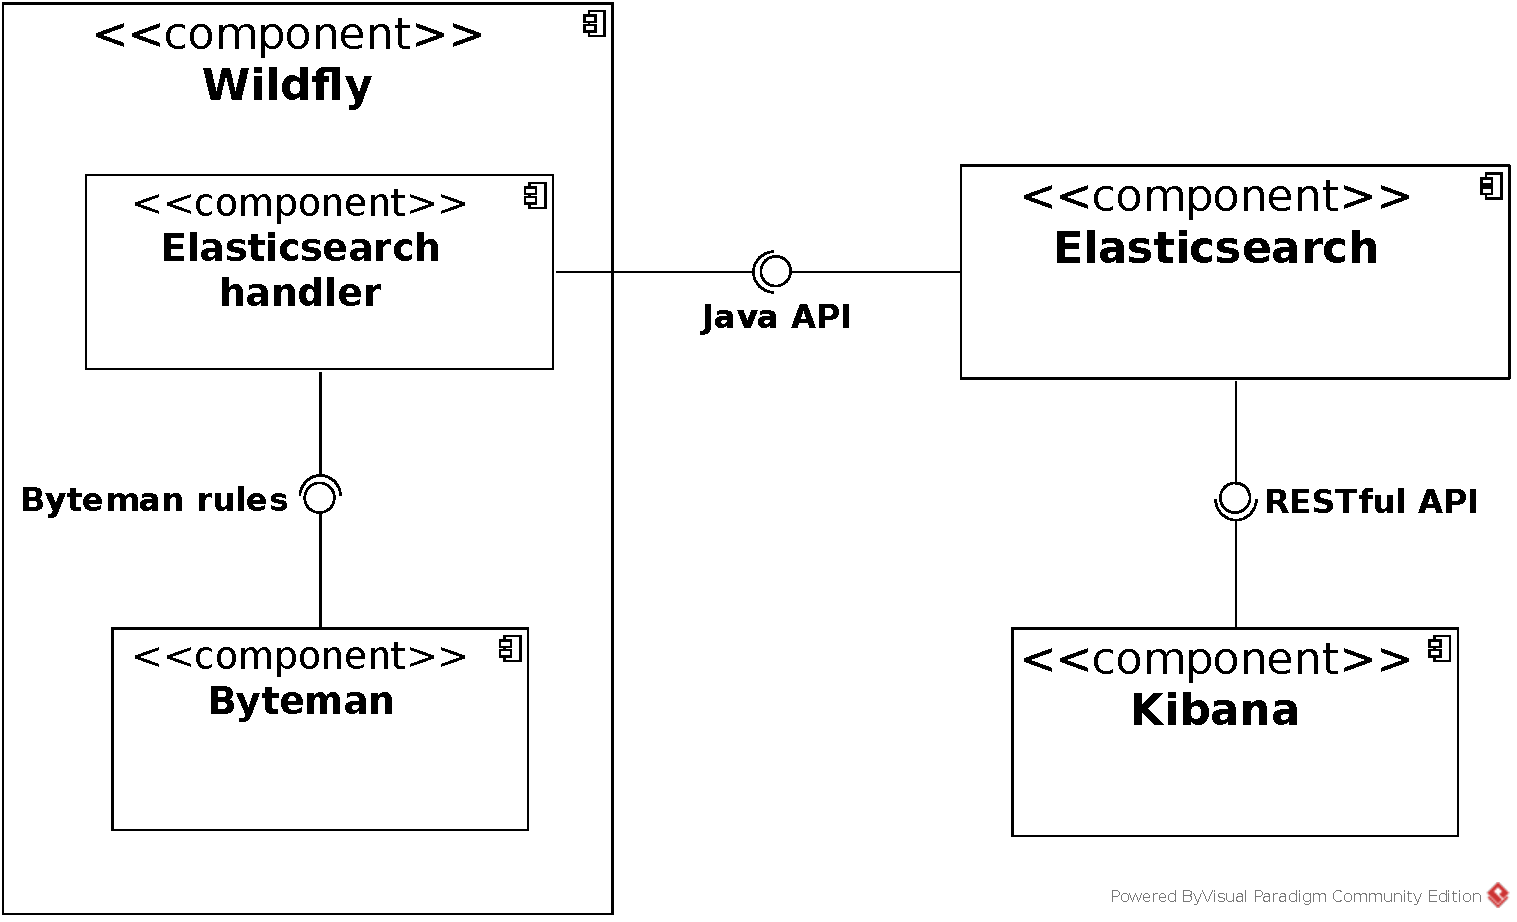
\includegraphics[width=\textwidth]{images/component_diagram}
	\caption{Component diagram}
	\label{component_diagram}
\end{figure}

\section{Tools}
This section introduces set of tools and technologies used for the implementation of the logging extension. Byteman and Elasticsearch are not mentioned in the following text as they are described in chapters \ref{byteman_chap} and \ref{elasticsearch_chap}. According to the nature of the Wildfly project, all tools and technologies should meet the following requirements:

\begin{itemize}
	\item Wildfly is \textit{Open Source}, thus only Open Source technologies should be used for the implementation
	\item Wildfly is implemented in the \textit{Java} language, this fact must be taken in consideration when choosing appropriate technologies
\end{itemize}

\subsection{IDE}
Effective development of any project should use an Integration Development Environment. It consists of several tools which help developer with fast and effective development. Such tools include text editor, debugger, build system, version control system and others. Eclipse is free Open Source IDE for Java. It uses plugins for integration with technologies such as Maven, Git, Wildfly and many JBoss projects. In addition, Red Hat JBoss Developer Studio can be used as it is built on top of Eclipse and includes plugins for JBoss technologies by default.

\subsection{Maven}
Development of an Java application requires an automation process for building the source code of the application. Maven is leading build automation tool for Java based projects. This work uses several aspects of Maven which are described in the following text.

To build a project with Maven, a project must define its project object model and set of plugins which are shared across all projects using Maven. The project object model is defined by the \textit{pom.xml} file which is a part of every Maven project \cite{maven_doc}. 

A Maven project must define its unique identification which consists of: \textit{groupId}, \textit{artifactId} and \textit{version}. This identification is defined within the \textit{pom.xml} file which also contains all configuration properties e.g. packaging (default is \textit{JAR}), project name, description and any custom properties defined by a user.

One of the most important elements in Maven are \textit{dependencies}. It provides comprehensive administration of libraries used in a Maven project. Libraries represents Maven projects which were published in a Maven repository. A dependency is defined by its unique identification (groupId, artifactId, version) and the dependency scope\footnote{Dependency Scope defines certain limitations when processing a dependency.}. Dependencies are downloaded from a remote Maven repository during the build process of a Maven project.

Maven repositories are defined in the \textit{settings.xml} file which is created after installing Maven on a user machine. Maven provides access only to the \textit{Maven Central Repository} by default, thus other repositories must be specified within the \textit{settings.xml}. In addition, a user can create its own repository which can be added to the \textit{settings.xml} as any other public repository.

\subsection{Git}
Version control system (CVS) provides necessary functions for software development such as history of changes, resolving conflict within same file and others. Main characteristic of the Git CVS is strong support for distributed development. For instance, each developer uses its local repository for work, thus changes are committed to a local repository at first, then pushed to a remote repository. In order to provide web-based service for Git repositories, the Github\footnote{https://github.com/} was created. It allows user to manage its repositories via web interface.

\subsection{Kibana}
Elasticsearch stores large amount of data that user needs to work with. Kibana allows user to search, view and analyze data within the Elasticsearch. It represents simple web interface for browsing data in real time. Moreover, Kibana provides advanced data analysis and visualization using various charts, tables and maps \cite[Introduction]{kibana_doc}. Note that installing and running Kibana does not require any additional implementation on the client side, thus using Kibana is very simple and intuitive.

\subsection{Bytecode manipulation tools}
The non-functional requirement of this work is to use an approach which allows user to add log events to Wildfly and does not change its source code. The Wildfly source code is written in Java language and compiled into bytecode. Thus, new log events must be added only by modifying the Wildfly bytecode, whereas the current source code is left untouched. To fulfill such requirement, the bytecode manipulation must be employed. There are several bytecode manipulation tools depending on the level of abstraction they use. The following picture shows selected tools and level they operate on:
\begin{figure}[ht!]
	\centering
	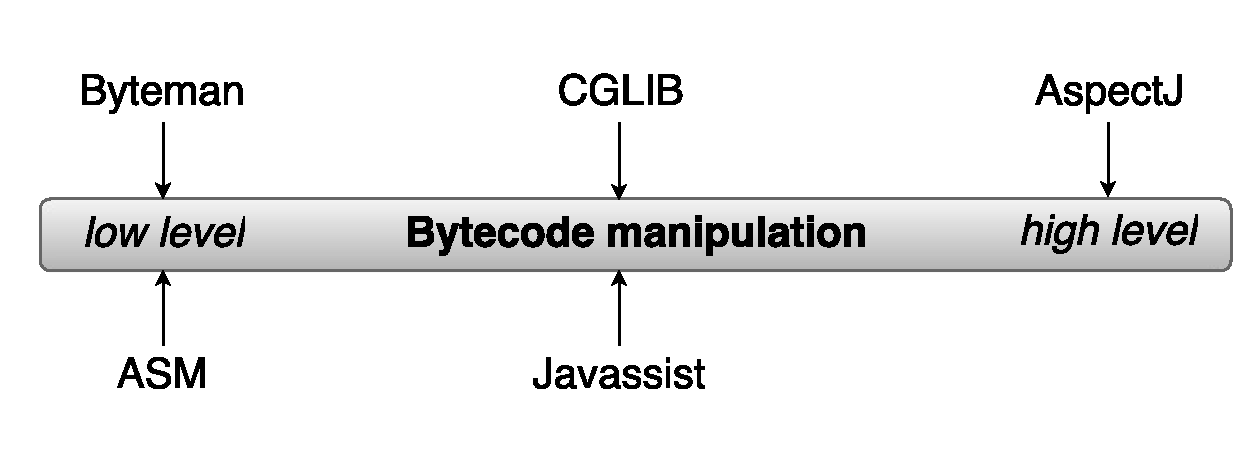
\includegraphics[width=\textwidth]{images/bytecode_tools}
	\caption{Bytecode manipulation tools}
	\label{bytecode_tools}
\end{figure}

Choosing a suitable bytecode manipulation tool is critical decision as all additional log events are implemented using the selected tool. Thus, replacing one tool with another requires rewriting the source code, which is not trivial operation in case of large number of log events. Selection of a bytecode library does not depend only on the architecture of the library itself, it also requires analysis of the library used against an application server which can be implemented in various ways. For instance, Wildfly application server uses modular classloading system \ref{jboss_modules_sec} that can cause classloading problems with specific bytecode library. Another requirement on the selected bytecode library is reusability of the implemented log events across different releases of Wildfly. For this reason, the bytecode library should provide bytecode analysis which is able to target specific parts within bytecode based on class names, method names, method invocations, variable assignments, constructor invocations and others.

The following bytecode manipulation tools were chosen for analysis and testing: \textit{Byteman} and \textit{AspectJ}\footnote{\url{https://eclipse.org/aspectj/}}. There is significant distinction between Byteman and AspectJ as they use different approach for bytecode manipulation. Byteman is a low level library which requires work at bytecode level, whereas AspectJ uses Java classes to achieve manipulation with bytecode. After appropriate analysis based on documentation and testing of selected tools, Byteman is used by the following reasons:

\begin{itemize}
	\item Byteman uses simple and powerful mechanism (see \ref{subsec:eca_sec}) to perform bytecode manipulation 
	\item AspectJ requires additional configuration using \textit{.xml} files for defining and working with aspects \cite[Configuration]{aspectj_doc}
	\item Byteman Rule Language \ref{byteman_rule_language} provides comprehensive bytecode analysis \ref{subsec:rule_events} to identify target location within bytecode
	\item in contrast to Byteman, AspectJ does not allow to manipulate with Java language classes defined in the \textit{java.lang} package \cite[Special cases]{aspectj_doc}
	\item Byteman provides set of built-in operations \ref{built-in_calls} which can be used for debugging, monitoring and thread coordinating purposes, thus user does not have to implement such operations for specific requirements
	\item both Byteman and Wildfly are part of the \textit{JBoss Community}\footnote{JBoss Community is a community of open source projects.}, this fact can simplify co-operation between developers in case of additional requirements
\end{itemize}

\chapter{Implementation}
This chapter describes implementation of the extended Wildfly logging capabilities in detail. The logging extension is split into two Maven projects:

\begin{itemize}
	\item \textit{elasticsearch-wildfly-log}: extension for Elasticsearch
	\item \textit{byteman-wildfly-log}: addition of new log events using Byteman
\end{itemize}

Both Maven projects are completely independent and can be used separately.

\section{Elasticsearch Wildfly Log}
Main functionality of the Elasticsearch Wildfly Log project is to store log events to Elasticsearch. This project is deployed as a static module in Wildfly. Thus, the project is built as a directory, which corresponds to the JBoss Module hierarchical directory structure depicted in figure \ref{jboss_modules_image}. The output directory has the following structure:

\begin{lstlisting}[caption = Elasticsearch Wildfly Log module directory structure, label = elasticsearch_module_structure]
org
|--elasticsearch
|   |--main
|      |--elasticsearch-1.6.0.jar
|      |--lucene-core-4.10.4.jar
|      |-- ... rest of Lucene jars
|      |-- module.xml
|--wildfly
    |--elasticsearch
       |--log
          |--main
             |--elasticsearch-wildfly-log-0.0.1-SNAPSHOT.jar
             |--module.xml
\end{lstlisting}

\noindent
Note that there are two modules in the output directory as the \textit{org.wildfly.elasticsearch.log} module requires Elasticsearch jars which are included in the separate module located in \textit{org.elasticsearch} subdirectory.

The storing process of log events includes several steps which are implemented in the \textit{ElasticsearchHandler} class. At first, the handler must establish a connection with an Elasticsearch cluster. To create such connection, a user must specify valid \textit{cluster name}, \textit{transport address} and \textit{port}.
If correct configuration is provided, the handler implementation uses the \textit{Transport Client} \ref{transport_client} to connect to a running cluster.

The next step in the storing process is to serialize a log event to the JSON format, which is used for data stored in Elasticsearch. The JSON format of the log event is designed to provide comprehensive data structure in order to support search operations in Elasticsearch.

\begin{lstlisting}[caption = JSON format of a log event, label = json_log_event]
{
 "timestamp":"timestamp",
 "jboss.bind.address":"server address",
 "jboss.server.name":"server name",
 "level":"log level",
 "loggerName":"loger name",
 "message":"log message",
 "thrown":{
  "name":"throwable name",
  "message":"throwable message"
 }
}
\end{lstlisting}

Note that the \textit{jboss.bind.address} and \textit{jboss.server.name} are obtained from Wildfly system properties. Information about server name and address is important in case of multiple server instances (e.g. cluster or cloud installation).

When a log event is successfully converted to the JSON format, transport client sends the log event to the Elasticsearch cluster which inserts received data into specific \textit{index} and \textit{type}. Index and type are defined by user when configuring the Elasticsearch handler in Wildfly logging subsystem (see \ref{logging_subsystem}).

\section{Byteman Wildfly Log}
This project is comprised of tools which provide bytecode manipulation in order to inject new log events into Wildfly bytecode. There are two main elements which forms the logging mechanism: \textit{LogHelper} class and \textit{Byteman rule script} files.



\bibliographystyle{IEEEtran}
\bibliography{sources}
\end{document}
